%%
%  ******************************************************************************
%  * #file    Szablon_raportu_EN_Latex.tex
%  * #author  Adrian Wójcik   adrian.wojcik(at)put.poznan.pl
%  *          
%  * #commit  Patryk Kościk   koscikpatryk(at)gmail.com
%  *          Modified the template for Projekt przejsciowy purposes          
%  *          
%  * #version 1.0
%  * #date    09-Mar-2022
%  * #brief   PROJPRZEJ
%  *
%  ******************************************************************************
%%  
\documentclass[11pt, a4paper]{article}

\usepackage{SM_template}

% Wypełnijcie te dyrektywy zgodnie z waszym tematem
% \lab      -> NAZWA CZUJNIKA, np.: 'DHT22'
% \comment  -> Króciutki opis co to, np.: 'Cyfrowy budżetowy czujnik temperatury'
%

\lab{Moduł KY-013}
\comment{Analogowy czujnik temperatury otoczenia}
\author{Antoni Borowski}
\addbibresource{bib/KY-013.bib}

% Absolutny zakaz dotykania tego tutaj bo jak dotkiecie to coś jebnie
\university{Politechnika Poznańska}
\faculty{Wydział Automatyki, Robotyki i Elektrotechniki}
\institute{Instytut Robotyki i Inteligencji Maszynowej}
\department{Zakład Sterowania i Elektroniki Przemysłowej}

\nocite{*}


%%
%
% Początek dokumentu
%
%%
\begin{document}

%% Strona tytułowa %%
\mainpage{{KY-013/foto}}
\newpage

\section*{Opis elementu} \addcontentsline{toc}{section}{Wstęp}
Czujnik KY-013 składa się z termistora NTC, wbudowanego rezystora 10k $\Omega$ oraz trzech pinów męskich. Termistor jest rezystorem półprzewodnikowym o rezystancji silnie zależnej od temperatury (w dużo większym stopniu niż w przypadku standardowych oporników). Rezystancja zmienia się w zależności od temperatury otoczenia. 
\vspace{0.5cm}
\begin{figure}[h!]
\centering
\begin{subfigure}{.5\textwidth}
  \centering
  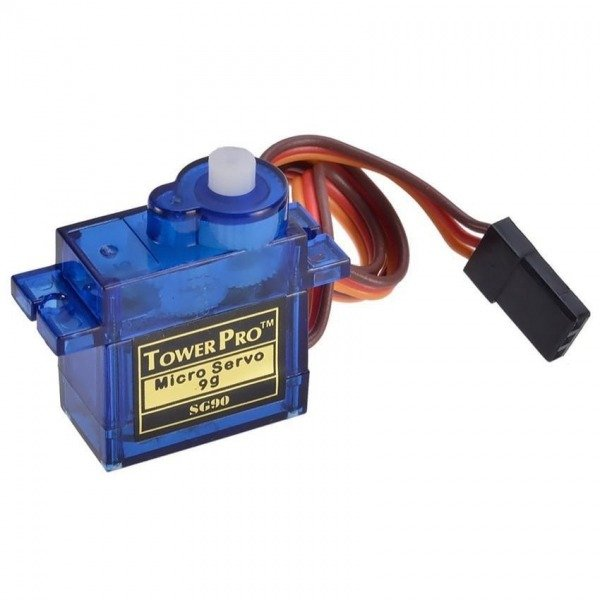
\includegraphics[width=.34\linewidth]{fig/KY-013/zdj_modułu/fig1.png}
  \caption{Moduł KY-013 \cite{ArduinoModules:Switch}}
  \label{fig:sub1}
\end{subfigure}%
\begin{subfigure}{.5\textwidth}
  \centering
  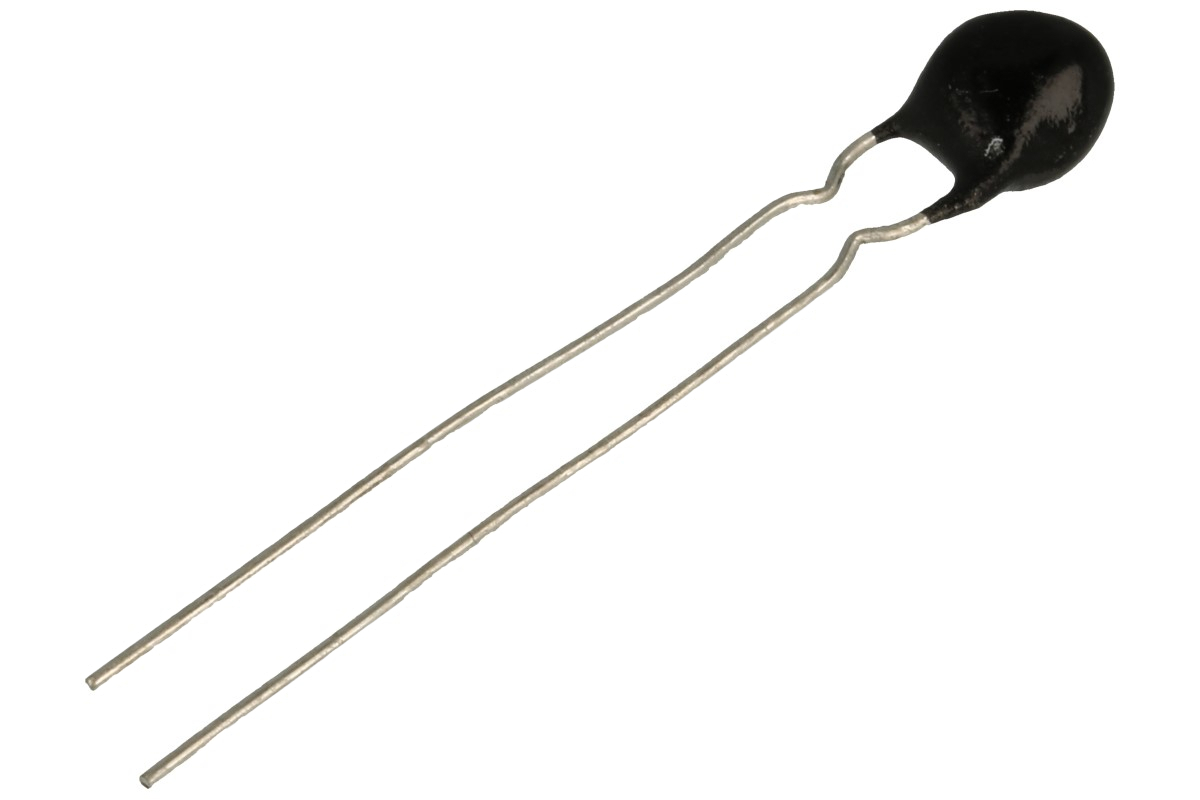
\includegraphics[width=0.94\linewidth]{fig/KY-013/zdj_modułu/fig2.jpg}
  \caption{Termistor \cite{ArduinoModules:grab}}
  \label{fig:sub2}
\end{subfigure}
\caption{Poglądowe rysunki modułu oraz termistora}
\label{fig:test}
\end{figure}

Termistor NTC płynnie zmniejsza rezystancję między swoimi wyprowadzeniami, kiedy temperatura otoczenia rośnie. Jest to możliwe dzięki zjawisku generacji termicznej, czyli samoistnemu rozpadaniu się wiązań między atomami budujących strukturę krystaliczną pod wpływem temperatury. Powstaje wtedy para elektron-dziura, swobodne nośniki prądu elektrycznego.

\begin{figure}[h!]
\centering
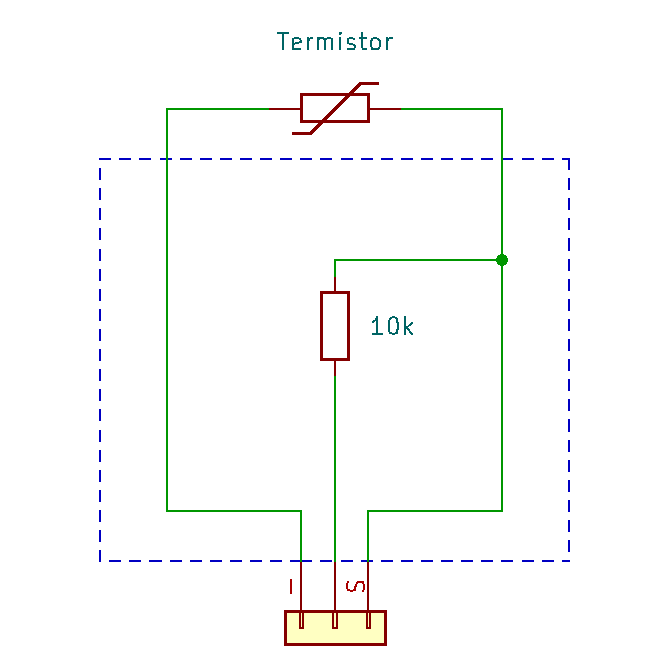
\includegraphics[width=.55\linewidth]{fig/KY-013/zasada_dzialania/schemacik.png}
\caption{Schemat modułu}
\label{fig:sub2}
\end{figure}

\newpage
\section*{Użycie czujnika}
Te czujniki temperatury działają jako element pasywny w obwodzie. Są precyzyjnym, tanim i wytrzymałym narzędziem do pomiaru temperatury. Chociaż nie działają dobrze w ekstremalnie wysokich lub niskich temperaturach, to wciąż posiadają wiele różnych zastosowań. Idealnie nadają się, gdy wymagany jest precyzyjny odczyt temperatury. Są powszechnie stosowane do pomiaru temperatury cieczy i powietrza otoczenia jako termometry termistorowe. Zastosowanie termistorów możliwe najczęściej jest w termostatach czy innych urządzeniach domowego użytku, jak piekarniki i lodówki.
\vspace{0.5cm}

Poniżej przedstawiono podstawową implementację czujnika na płytce stykowej.

\vspace{0.5cm}
\begin{figure}[h!]
    \centering
    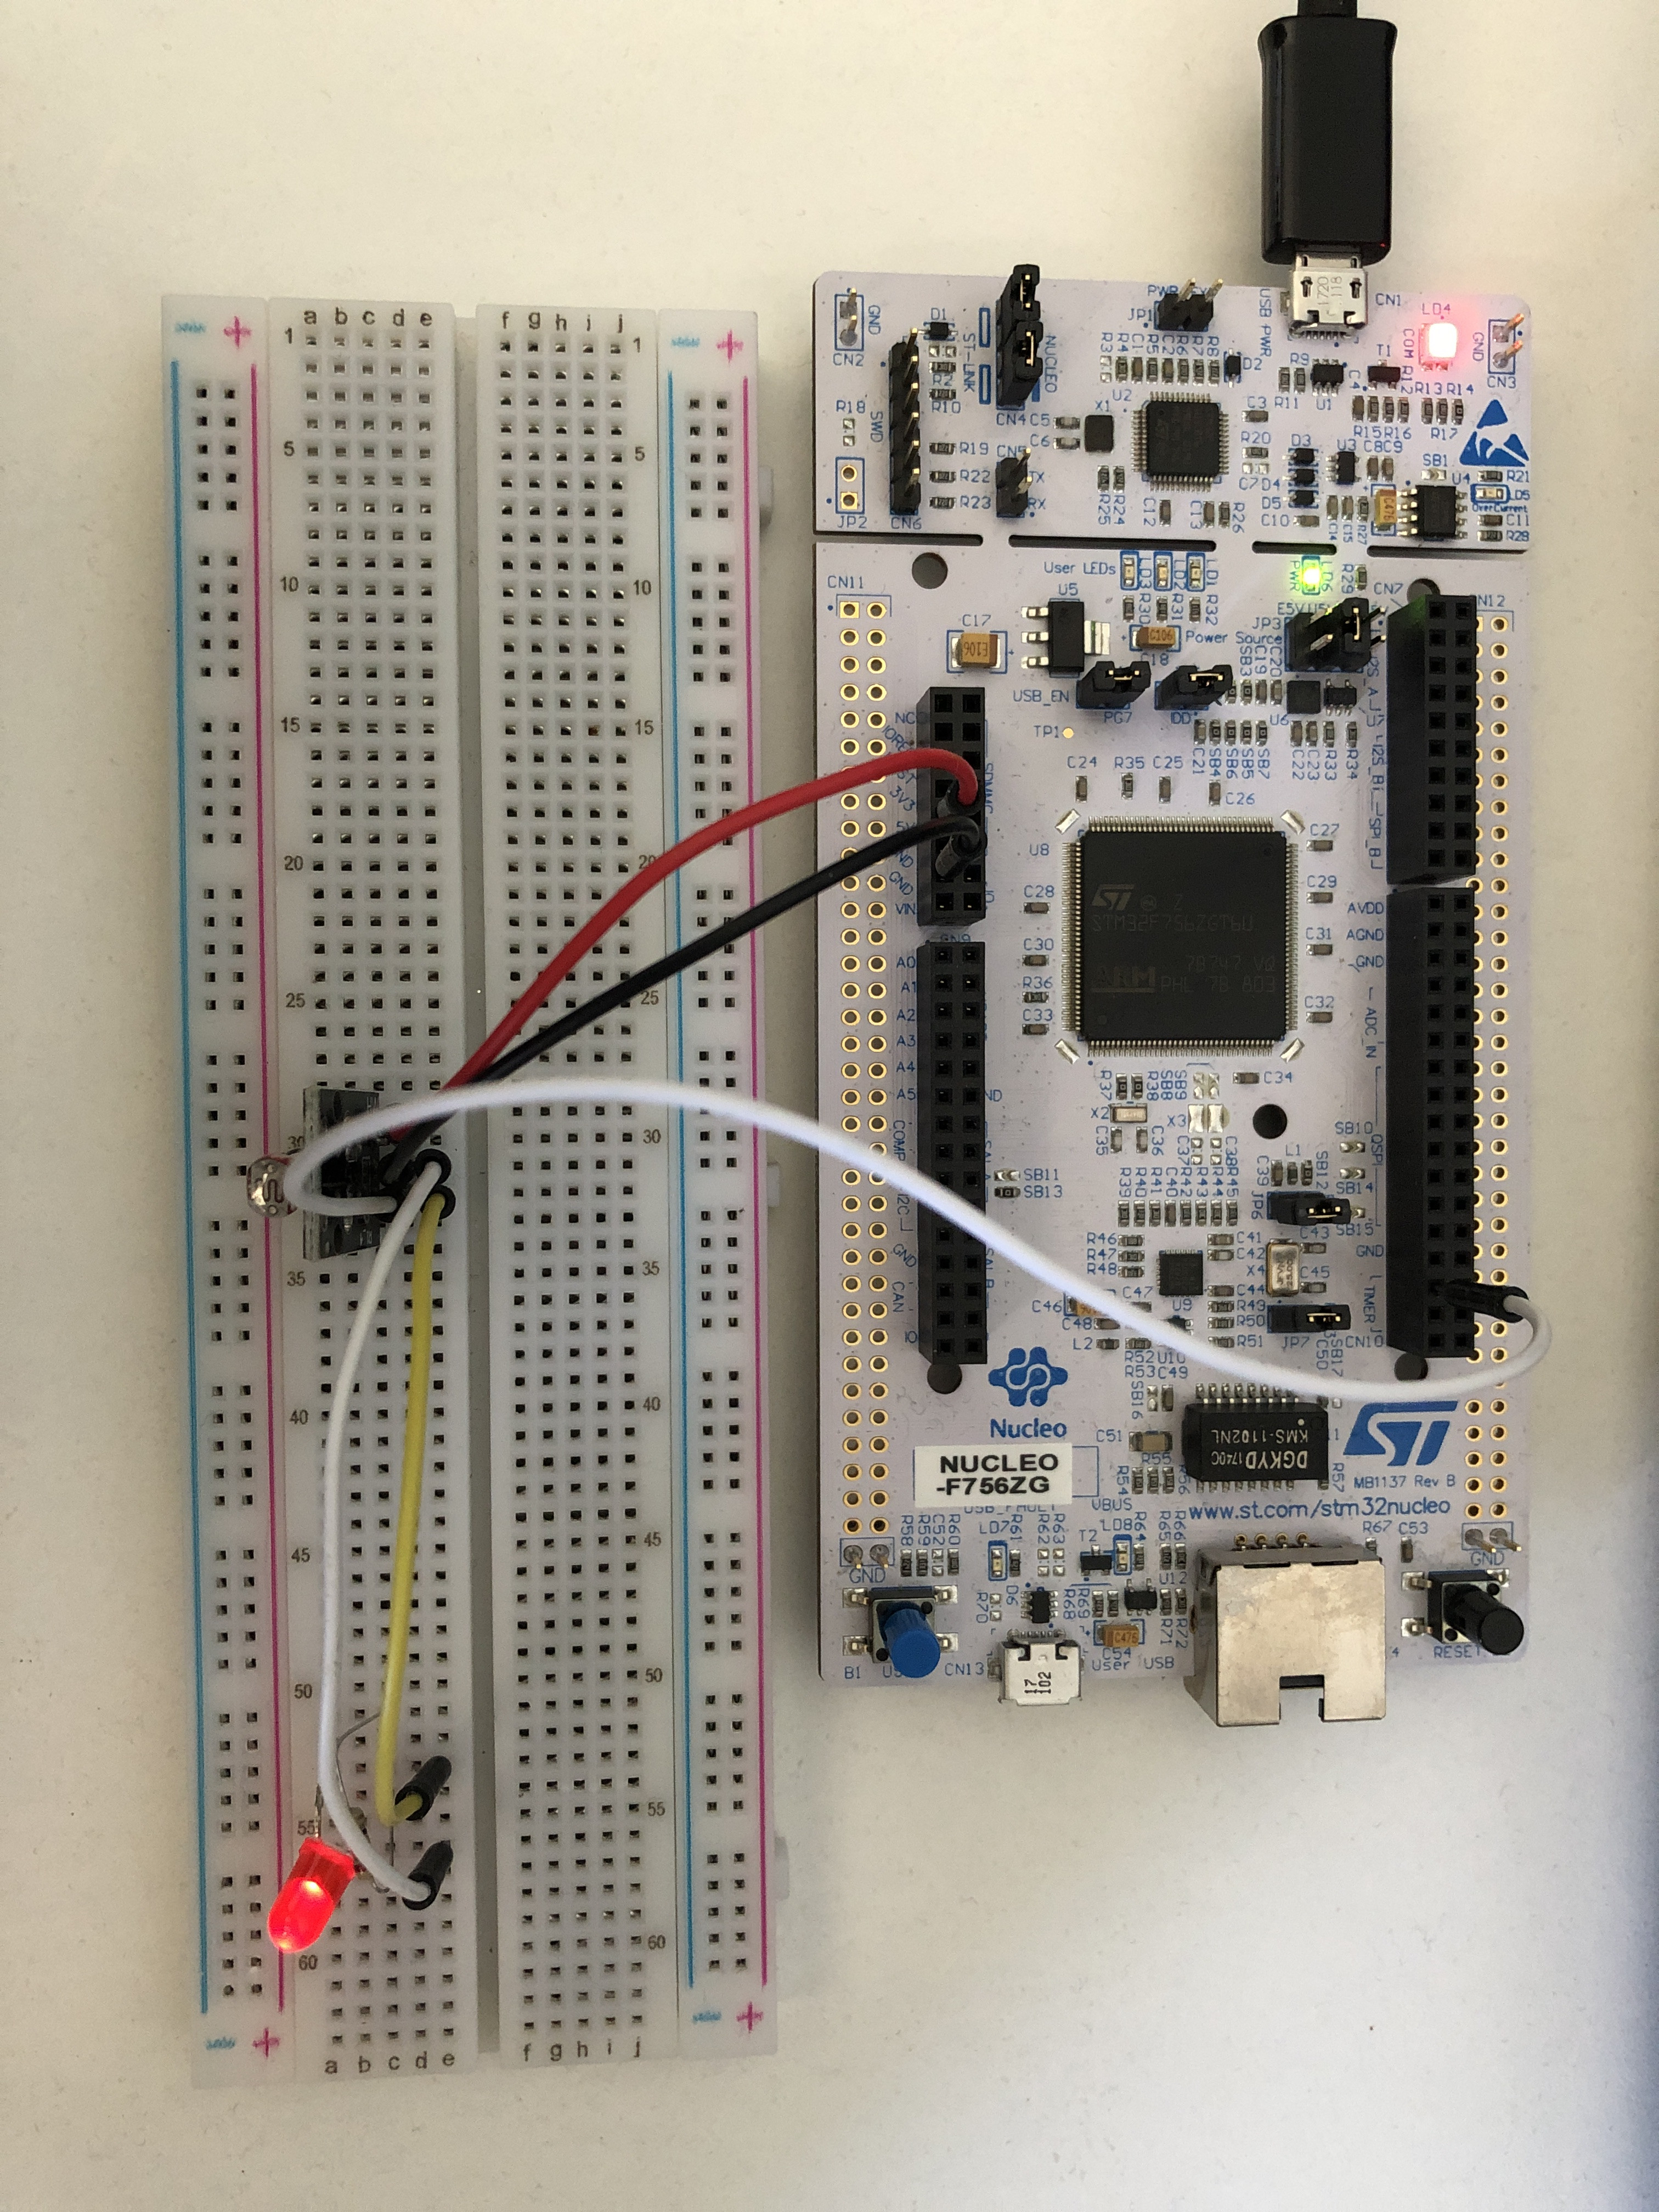
\includegraphics[width=0.3\textwidth,angle=90]{fig/KY-013/działanie_ukladu/final.jpg}
    \caption{Podłączenie modułu}
    \label{fig:my_label}
\end{figure}

Na Rys.3 termistor jest w temperaturze pokojowej, jego rezystancja jest niska, dzięki czemu dioda się świeci.

\vspace{0.5cm}

\begin{figure}[h!]
    \centering
    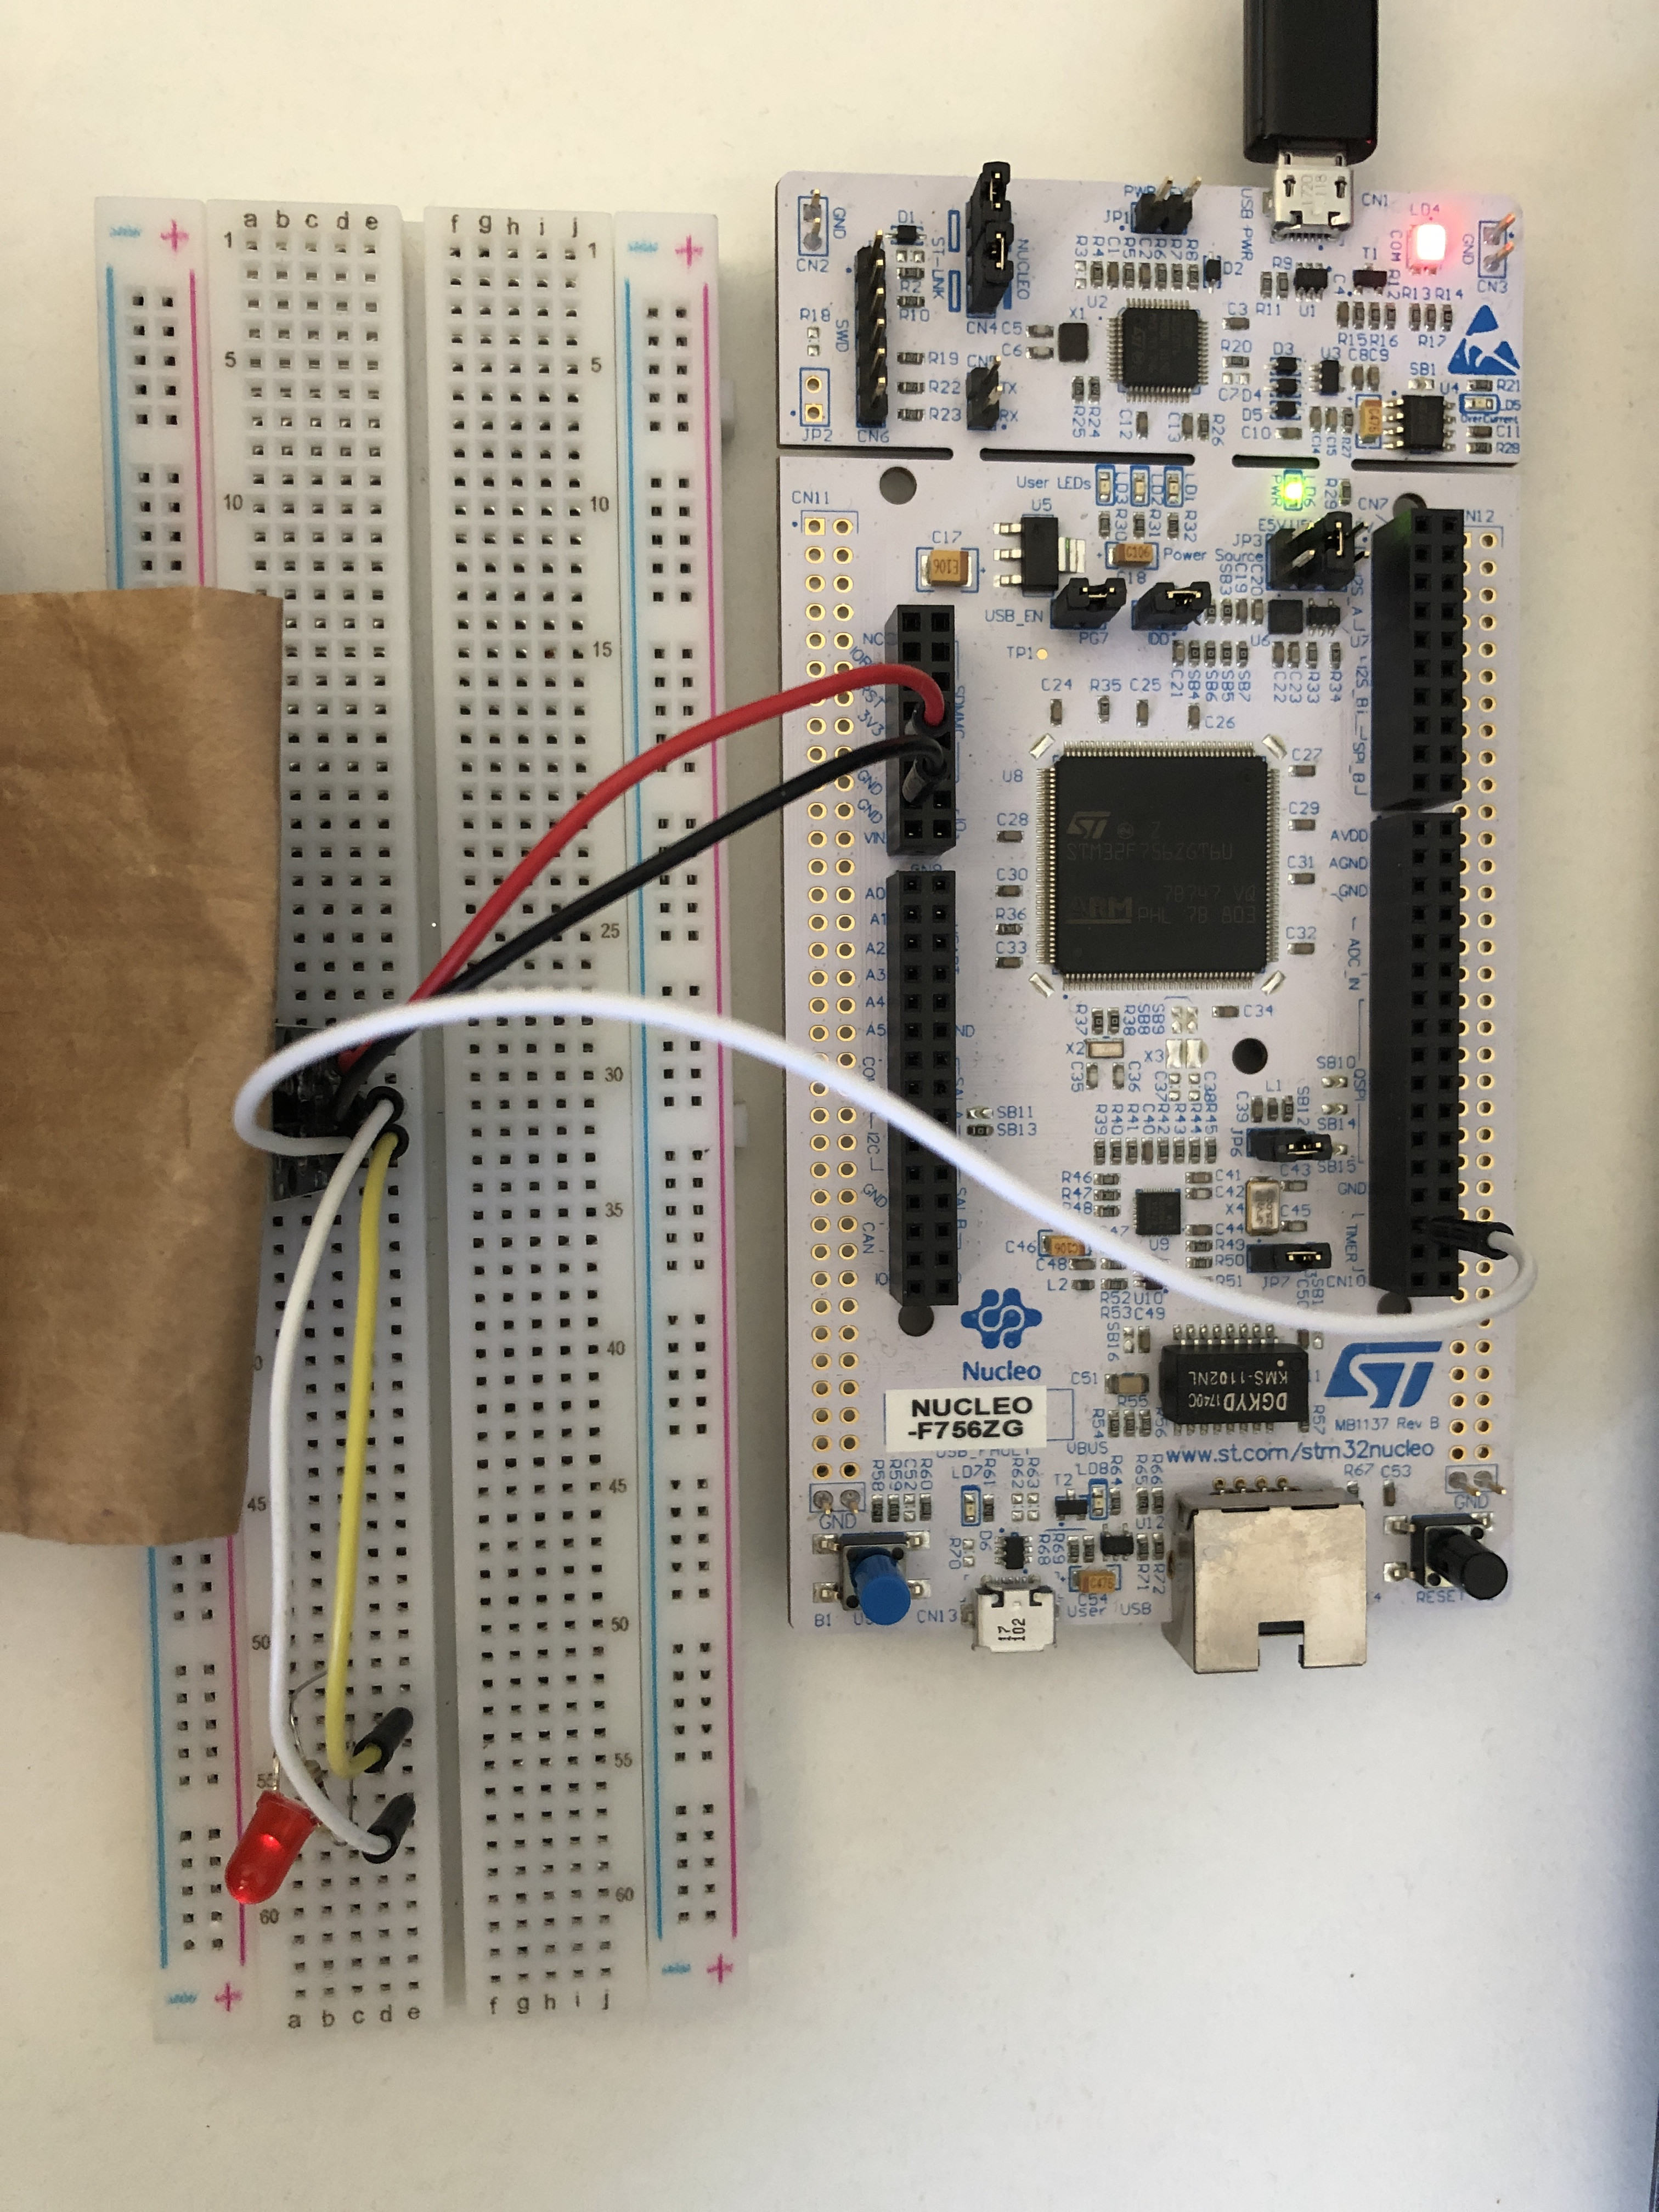
\includegraphics[width=0.3\textwidth,angle=90]{fig/KY-013/działanie_ukladu/final2.jpg}
    \caption{Podłączenie modułu}
    \label{fig:my_label}
\end{figure}

Na Rys. 4 do termistora zostało przyłożone źródło ciepła - rezystancja termistora drastycznie wzrasta, przez co dioda podłączona do modułu przestaje świecić.

\newpage 

Kod programujący czujnik, wykorzystany do opracowania instrukcji, znajduje się w materiałach dodatkowych zawartych pod koniec rozdziału.
\newline
Film prezentujący działanie układu znajduje się w suplemencie wideo.
\printbibliography[heading=bibintoc]

\end{document}